\section{Heat conduction with source term}
\label{sec_source_term}

In this section, we move a step forward, and solve a steady heat
conduction problem, but with the addition of source term.
This problem is governed by the equation:
%
\be
         \int_S \lambda \nabla T \, d{\bf S}
       = \int_V \dot{q} \, dV     
       \; \; \; \;
       [W]
  \label{eq_source_term}
\ee
%
Let's consider the same computational domain as in~Sec.~\ref{sec_conduction}
with following boundary conditions:
%
\begin{itemize}
  \item $T = 300 \; [K]$ at $x = 0$ and $x = 1$,
  \item $\frac{\p T}{\p n} = 0$ everywhere else. 
\end{itemize}
% 
and let's set the internal heat source to $\dot{q} = 100.0 \; [\frac{W}{m^3}]$.
It is straightforward to work out the analytical solution to this problem:
%
\be
  T(x) = \frac{\dot{q}}{2 \lambda} (x^2-x) + 300 \; \; \; \; \; [K]
  \label{eq_source_term_solution}
\ee
%
It is a parabolic temperature profile, reaching the maximum of $T = 312.5 \; [K]$
at $x=0.5$.

The program which discretizes and solves this problem ({\tt 07-03-main.cpp})
is created by slight modifications of the pure heat conduction program 
({\tt 07-01-main.cpp}) and here we outline only the lines which differ
between these two programs:
%
{\small \begin{verbatim}
     ...
     18   t.bc().add( BndCnd( Dir::imax(), BndType::dirichlet(), 300.0 ) ); /* b.c. */
     ...
     37   t = 350.0;                                        /* initial "guess" */
     38
     39   for_vijk(q,i,j,k)                                 /* fill the source term */
     40     q[i][j][k] = 100.0 * q.dV(i,j,k);
     41
     42   multigrid.vcycle(ResRat(1e-4));                   /* solve linear system */
     ...
\end{verbatim}}
%
The change in line~18 is apparent: the boundary temperature at $i=i_{max}$ to~$300 \; [K]$
Source term for~Eq.~\ref{eq_source_term} is defined in lines~38 and~39. The macro 
{\tt for\_vijk(q,i,j,k)} in line~38, should be familiar - it browses through all internal cells of
{\tt Scalar q}, but line~39 deserves special attention. Since {\psiboil} discretizes equations
in their {\em integral} form (see Sec.~\ref{sec_equations}), the source term (i.e.\ the right
hand side) of the discretized equation must also be in integral form. That is why we multiply
prescribed value of internal heat source ($100 \; [\frac{W}{m^3}]$) with cell volume ({\tt q.dV(i,j,k)})
in each cell. We actually apply mid-point integration rule to have the source term in
right dimensions, which is, for case of enthalpy equation a~$[W]$. 

The solution obtained by the program {\tt 07-03-main.cpp} 
is given in Fig.~\ref{fig_temperature_source}. The temperature profile is parabolic in $x$
direction, and reaches maximum of $T = 312 \; [K]$ at $x=0.5$, as predicted by analytical
solution in~Eq.~\ref{eq_source_term_solution}.

%---------------%
%               %
%  Temperature  %
%               %
%---------------%
\begin{figure}[ht]
  \centering
  \setlength{\unitlength}{1mm}
  \begin{picture}(100,85)(0,0)
    \thickbox{100}{85}
    \put(0,-3){\includegraphics[scale=0.45]{Figures/07-03-temp.eps}}
  \end{picture}
  \caption{Temperature field solution for steady conduction with heat source.}
  \label{fig_temperature_source}
\end{figure}

\subsection{Changing the physical properties}

The solution of steady heat conduction without source terms, did not depend on
physical properties of the material under considerations. But, for steady heat 
transfer with source term (Eq.~\ref{eq_source_term}) solution depends on
thermal conductivity $\lambda$. We did not specify anything for it in the
program {\tt 07-03-main.cpp}, meaning that {\psiboil} used the default 
values, which is $1$. To set it to different value, say $\lambda = 2.0$, the
following command should be used:
%
{\small \begin{verbatim}
          solid.lambda(2.0);
\end{verbatim}}
%
after {\tt Matter} has been defined and before the definition of the
governing {\tt Equation}. 
%
Modify the program {\tt 07-03-main.cpp} to define  $\lambda = 2.0$. 
Re-compile and re-run. Numerical solution should reach maximum $T = 325 \; [K]$. 

Other {\tt Mater}'s member function, which can be used to change physical properties 
are:
%
\begin{itemize}
  \item {\tt Matter::rho   (real value);} - density              $\rho \; [\frac{kg}{m^3}]$
  \item {\tt Matter::mu    (real value);} - dynamic viscosity    $\mu \; [\frac{kg}{m \, s}]$
  \item {\tt Matter::cp    (real value);} - thermal capacity     $C_p \; [\frac{J}{kg \, K}]$
  \item {\tt Matter::lambda(real value);} - thermal conductivity $\lambda \; [\frac{W}{m \, K}]$
  \item {\tt Matter::gamma (real value);} - specified diffusivity  $\gamma \; [\frac{kg}{ms}]$ 
  \item {\tt Matter::sigma (real value);} - surface tension      $\sigma \; [\frac{N}{m} = \frac{kg}{s^2}]$
\end{itemize}

%---------------------------------------------------------------------nutshell-%
\vspace*{5mm} \fbox{ \begin{minipage}[c] {0.97\textwidth} %-----------nutshell-%
    {\sf Section \ref{sec_source_term} in a nutshell} \\  %-----------nutshell-%
   
      - When specifying a source term, make sure it has right dimensional
      units. \\ 

      - Keep in mind that {\psiboil} solves transport equations in
      {\em integral} form. \\

      - It is almost sure that you will have to integrate the prescribed
      source term with the mid-point rule (multiplying it by cell volume) \\

      - Use {\tt for\_vijk(Scalar,int,int,int)} macro to browse through source 
      field and member function {\tt Scalar::dV(i,j,k)} to access cell volume. \\

      - Physical properties can be set by {\tt Matter}'s member functions.

  \end{minipage} } %--------------------------------------------------nutshell-%
%---------------------------------------------------------------------nutshell-%
